


\documentclass[12pt,a4paper]{book}



			% Packages Files
%----------------------------------%

	% Page Setttings
\usepackage[top = 1in, bottom = 1in, left = 1in, right = 1in]{geometry}

\parindent=0cm % to prevent the spacing in new paragraph or new line

\usepackage{fancyhdr}
\setlength{\headheight}{14.5pt} % needded for header and footer 

%-----------------------------------------------------------------%

\usepackage{amsmath} % needed for referencing thequation
\usepackage{amsfonts} % for maths symbols
\usepackage{graphicx}
\usepackage[export]{adjustbox}
\usepackage{nomencl} % must be loaded before caption (KOMA tocbasic conflict)
\usepackage{caption}
\usepackage{refstyle} % to reference a captioned figure


% To make hyperlinks

\usepackage[
	colorlinks=true
	,breaklinks
	]{hyperref} % needed for creating hyperlinks in the document, the option colorlinks=true gets rid of the awful boxes, breaklinks breaks lonkg links (list of figures),
	
\usepackage{xcolor}
\definecolor{c1}{rgb}{0,0,1} % blue
\definecolor{c2}{rgb}{0,0.3,0.9} % light blue
\definecolor{c3}{rgb}{0.3,0,0.9} % red blue
\hypersetup{
    linkcolor={c1}, % internal links
    citecolor={c2}, % citations
    urlcolor={c3} % external links/urls
}

	% For Code Writing
	
\usepackage{listings}

\usepackage{color}

\definecolor{mygreen}{rgb}{0 0.6 0}

\lstset{
% Set automatic Line breaking, in case we have long lines don't
% fit inside the frame or the page.
breaklines = true,
commentstyle = \color{mygreen},
breakatwhitespace = true,% don't show white space character
%numbers = left, % put line number in the code
title = \lstname
}

% ------------- For Writing Equations inisde a table and centering them ------------

\usepackage{array}

% Vertical Alignment inside the cells of the table
\newcolumntype{M}[1]{>{\centering\arraybackslash}m{#1}}

% Horizontal Alignment inside the cells of the table
\newcolumntype{P}[1]{>{\centering\arraybackslash}p{#1}}


% needed for todos liste
\usepackage{todonotes} 



% %---------- needed for long tables over pages-------
\usepackage{longtable} 

\usepackage[acronym]{glossaries}




% Macros File

% Macros Example
\def\labelaxes{Remember to include some suitable labeling for the axes and the units used in measurements.}

% 2nd way for defnining macros: the new command
% 1st parameter: name of the new command
% 2nd paramter: how many inputs this command needs, in this case only 1
% 3rd parameter: what this new command named \tbi do

\newcommand{\tbi}[1]{\textbf{\textit{#1}}}

% Command for Picture without a label

\newcommand{\pic}[3]{\begin{figure}[h]
\centering
\includegraphics[width = 0.7\textwidth, frame]{#1}
\caption{#2}
\end{figure}}








\DeclareMathOperator*{\argmax}{argmax} % thin space, limits underneath in displays

\DeclareMathOperator*{\argmin}{argmin}

\title{Simulation for Sparsity and CS}
\author{Ranim Tom}



\begin{document}

% downloaded template
%\input{content/title_page_1} 

\maketitle
\tableofcontents

% to make the todo list appear as a table of content
\listoftodos


\pagestyle{fancy}
\fancyhf{} % Clear header and footer
\rhead{\rightmark}
\lhead{Chapter \thechapter}
\rfoot{Page \thepage}

\chapter{Greedy Algorithm}


\section{Perminilinary}

Before starting the examples, let's make a small recall about the problem formulation and notation used in CS problem.

The modeling of the CS problem is embedded via \autoref{Eq:Compressed_Sensing:formulation_2}

\begin{equation}
	\begin{array}{rcl}
 \Vec{y}_{m \times 1} \, &=& \, \boldsymbol A_{m \, \times \, n} \,\times \,  \Vec{x}_{n \times 1} \\ 
		 &=& \, \boldsymbol \Phi_{m \, \times \, n} \, \times \, \boldsymbol \Psi_{n \times n} \, \times \, \Vec{x}_{n \times 1}
	\end{array}
\label{Eq:Compressed_Sensing:formulation_2}
\end{equation}

where

\begin{itemize}
    \item $\boldsymbol A$: is the sensing matrix
    
    \item $ \boldsymbol \Phi$: measurement matrix
    
    \item $ \boldsymbol \Psi$: basis matrix
    
\end{itemize}

The $\Vec{x}_{n \times 1}$ is a sparse vector in some domain (frequency,time,$\cdots$). If it is not sparse we should \tbi{apply some sparse transformation}, like DFT to some time domain vector (as we will do in the example).\\


\section{Example 1: 3 Spike Component}


\underline{Source:} See section 3.2, example 1 in \cite{paper_tutorial_sparse_Stankovic}, and \cite{paper_numerical_toor} for extra examples and details for implementation (how to implement random matrices and do random selection).

\subsection{Preprocessing}

\begin{itemize}

\item A continuous time signal is being taken shown in \autoref{Eq:Example_Signal_CS}

\begin{equation}
    x(t) \, = \, 0.3 \, + \, 0.4 \exp(-j 12 \, \pi \, t) \, + \, 0.5 \, \exp(-j 50 \, \pi \, t)
    \label{Eq:Example_Signal_CS}
\end{equation}

\item The signal is being sampled at $F_s \, = \, 64$ Hz for 1 s duration, resulting in a total number of samples of 64

\item We choose number of measurement in \tbi{time domain} is $m \, = \, 16$, \tbi{taking randomly} 

\item Since is our initial sampled time domain signal is not sparse, we need to sparsify it, by applying a DFT transform $\rightarrow$ we obtain a sparse frequency signal

\item The random measurement will be taken in the time domain, so \autoref{Eq:Example_Signal_CS} is applied as follows (for illustration I take $m \, = \, 2$ and $n \, = \, 5$):

\begin{equation}
\begin{array}{lll}
 \Vec{y}_{m \times 1} \, &=& \, \boldsymbol A_{m \, \times \, n} \,\times \,  \Vec{x}_{n \times 1} \\ 
		 &=& \, \boldsymbol \Phi_{m \, \times \, n} \, \times \, \boldsymbol \Psi_{n \times n} \, \times \, \Vec{x}_{n \times 1} \\ \\
		 &=& \, \begin{bmatrix}
		 1 & 0 & 0 & \cdots & 0 \\
		 0 & 0 & \cdots & 1 & 0 \\
		 \end{bmatrix}_{m \times n}
		 \times \, \begin{bmatrix}
		 1 & 0 & 0 & \cdots & 0 \\
		 \vdots & \vdots & \vdots & \vdots & \vdots & \\
		 0 & 0 & 0 & \cdots & 0 \\
		 0 & 0 & \cdots & 1 & 0 \\
		 
		 0 & 0 & 0 & \cdots & 0 \\
		 \end{bmatrix}_{n \times n} \, \times \, \boldsymbol F^{-1}_{n \times n} \, \times \, \Vec{x}_{n \times 1}
		 
\end{array}
\label{Eq:Compressed_Sensing:formulation_2}
\end{equation}

Here, the measurement matrix $\boldsymbol A$ is \tbi{random inverse partial DFT matrix}.

Always remember that \tbi{measurement matrix}  $\boldsymbol A$ are \tbi{wide matrices}.

\end{itemize}

\subsection{Displaying Some Results}

In \autoref{fig:Sim_Sparse:OMP_Run_Sparse_Frequency_Nb_11}, we see a run trial using OMP algorithm (explained next section).


\begin{figure}[ht]
\centering
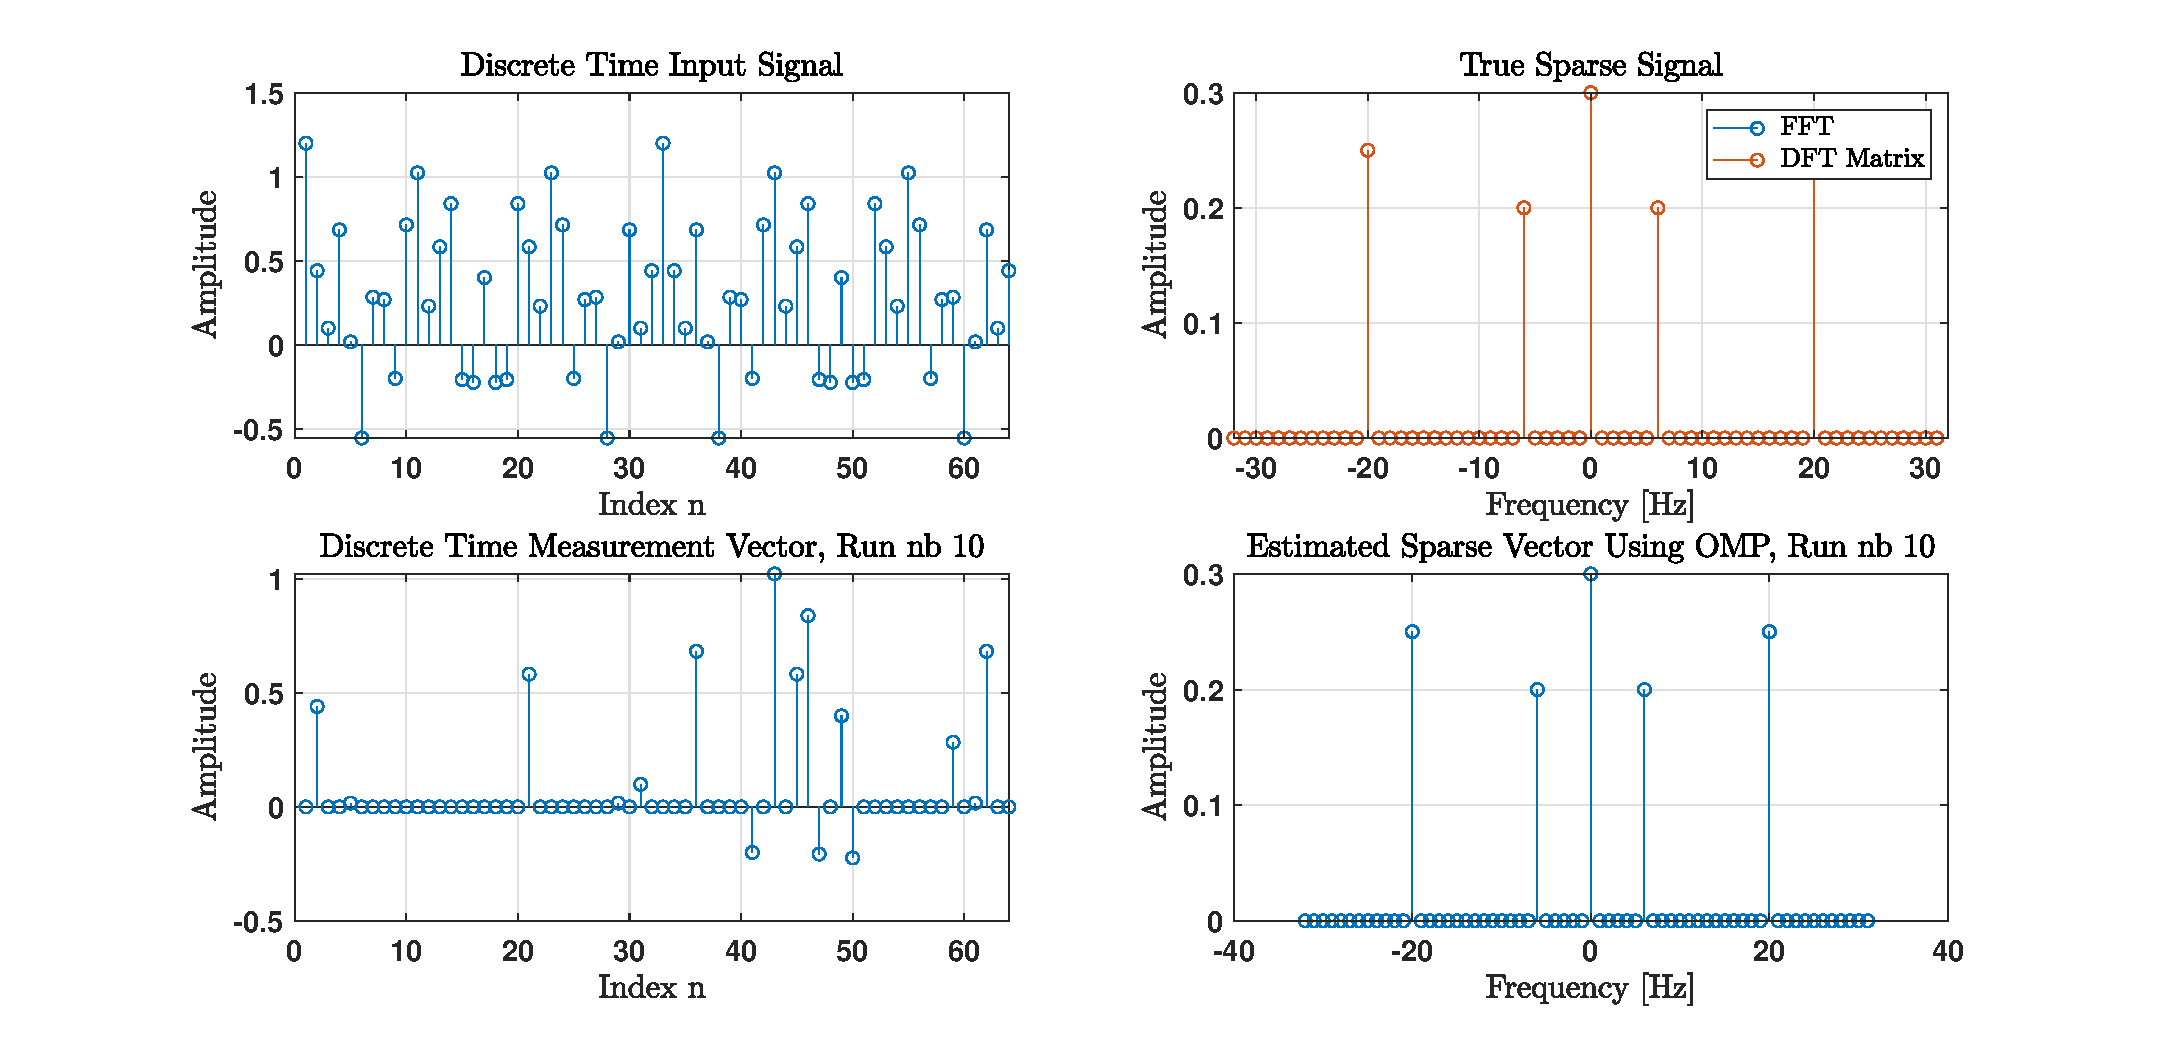
\includegraphics[width = 0.9\textwidth, frame]{Figures/Sim_Sparse/OMP_Run_Sparse_Frequency_Nb_11}
\caption{Simulation Output}
\label{fig:Sim_Sparse:OMP_Run_Sparse_Frequency_Nb_11}
\end{figure}

\begin{itemize}
    \item $\mathrm{1}^\mathrm{st}$ column: the sampled signal and the random measurement taken
    
    \item $\mathrm{2}^\mathrm{nd}$ column: the true sparse vector (implemented using and FFT and DFT) and the estimated one.
\end{itemize}


\subsection{OMP Explanation}

\todo{OMP Explanation}: 

\underline{\textit{OMP Explanation}:}\\ 

\textit{To explain it later with picture of matrices, update the measurement of matrix according to update support,$\cdots$}.\\

\textit{Use idea of slides of Michael Elad}. 

\begin{itemize}

\item OMP Algorithm:

\begin{enumerate}
    \item Search for the best atom in $\boldsymbol A$ that explain $ \Vec{y} \,  =  \, \boldsymbol A \Vec{x}$ 
    
    \begin{itemize}
        \item $\rightarrow \Vec{\rho} \, = \, \boldsymbol A^T \, \Vec{r}$, where $\Vec{\rho}$ is the correlation vector and $\Vec{r}$ is the residual vector
        
        \item Taking the index of the maximum value in $\Vec{\rho}$
        
    \end{itemize}
    
    
    \item Update the support of indices: $S_k: S_k \, = \, S_{k \, - \, 1} \, \displaystyle\cup \, \{ i_0\}$
    
    \item We solve for the values of $\Vec{x}_k$ subject to the updated indices, using a least square problem
    
      \begin{equation}
         \Vec{x}_k \, = \, \min_{\Vec{x}_k} \lVert A \, \Vec{x} \, - \, \Vec{y} \rVert_2 \quad \text{s.t } \text{ Supp} \{\Vec{x}\} \, = \,  S_k
     \end{equation}
    
    
    \item Update the $\Vec{r} \rightarrow \Vec{r} \, = \, \Vec{y} \, - \, \boldsymbol A \, \Vec{x}_k$
    
\end{enumerate}


\end{itemize}


\subsection{KPI}

As KPI, we can use the following:

\todo{KPI}

\textit{KPI}:

\textit{To redo them later with analysis. Maybe after finishing the algorithm here the analysis part of Elad}.


\begin{enumerate}
    \item Relative error:
    
    \begin{equation}
        \text{Error}_{L_2} \, = \, \displaystyle\frac{\lVert  \hat{\vec{x}} \, - \, \vec{x} \rVert_2^2 }{\lVert \vec{x} \rVert_2^2}
    \end{equation}
    
    
\item We can also asses support recovery based on the normalized intersection of the true and the estimated support by applying the following equation:

\begin{equation}
 \text{Error}_{S} \, = \, 1 \, - \, \displaystyle\frac{\lvert \hat{S} \rvert \, \cap \, \lvert S \rvert}{\max \left\{ \lvert \hat{S} \rvert \, , \,  \lvert S \rvert  \right\} }  
\end{equation}
 
If the 2 support don't overlap, their intersection is 0 and hence $\text{Error}_{S}$ is equal to 1
\end{enumerate}




%**************** References ****************

\bibliographystyle{IEEEtran}

\bibliography{Literature/Books_Signal_Processing,Literature/Papers_Sampling}


\end{document}





